% Information diagram of two random variables.
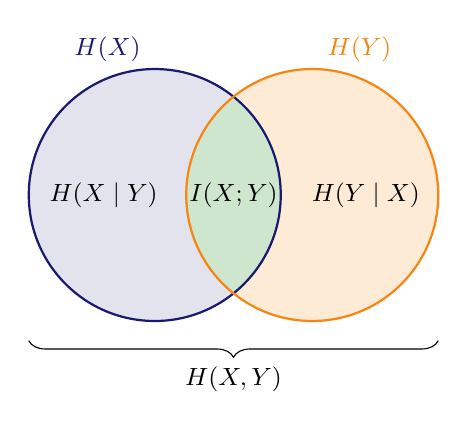
\begin{tikzpicture}[font=\small]
\fill[MidnightBlue!12] (0,0) circle (1.6);
\fill[BurntOrange!14] (2,0) circle (1.6);
\begin{scope}\clip (0,0) circle (1.6); \fill[ForestGreen!22] (2,0) circle (1.6); \end{scope}
\draw[MidnightBlue,thick] (0,0) circle (1.6);
\draw[BurntOrange,thick] (2,0) circle (1.6);
\node at (-0.65,0) {$H(X\mid Y)$};
\node at (1,0) {$I(X;Y)$};
\node at (2.68,0) {$H(Y\mid X)$};
\node[MidnightBlue] at (-0.6,1.85) {$H(X)$};
\node[BurntOrange] at (2.6,1.85) {$H(Y)$};
\draw[decorate,decoration={brace,amplitude=6pt,mirror}] (-1.6,-1.85) -- (3.6,-1.85) node[midway,below=6pt] {$H(X,Y)$};
\end{tikzpicture}
